\documentclass[letterpaper, 11pt]{article}

\usepackage[pdftex]{graphicx}
\usepackage{epstopdf}
\DeclareGraphicsRule{*}{mps}{*}{} 

\usepackage{amsmath, amsthm, amssymb}
\usepackage{listings}
\usepackage{float}
\usepackage{enumerate}
% \usepackage{mystyle}
\usepackage{hyperref}
\usepackage{tikz}
\usepackage{fancyheadings}
\usepackage{tensor}
\usepackage{mathrsfs}
\usetikzlibrary{positioning}
\usetikzlibrary{decorations.pathmorphing}
\usetikzlibrary{arrows}
\usetikzlibrary{decorations.markings}
%\usepackage{fullpage}
\usepackage[left=0.75in, top=1.25in, right=0.75in, bottom=1.25in]{geometry}
\newcommand{\lambdabar}{{\mkern0.75mu\mathchar '26\mkern -9.75mu\lambda}}

\numberwithin{equation}{section}
\numberwithin{figure}{section}

\begin{document}

\title{Numerical Methods for Astrophysical Magnetohydrodynamics}
\author{Jim Stone}
\date{July 19, 2016}

\maketitle

\section{Lecture 1 --- Astrophysical MHD}

I will mainly talk about one single class of numerical method for MHD, which is
finite volume method. Link to the \href{http://www.astro.princeton.edu/~jstone/downloads/papers/Lecture1.pdf}{slides}.

\subsection{Overview}

Why are we interested in doing numerical MHD? Most of the big questions in
astrophysics require the study of the dynamics of visible matter in the form of
plasma. For example, how do galaxies form, how do stars form, how do planets
form, etc. We are going to focus on collisionless plasma today, and for
collisional plasma additional methods are required.

The equations of inviscid ideal MHD are as follows (in units so that $\mu = 1$)
\begin{align}
  \frac{\partial\rho}{\partial t} + \nabla \cdot \left( \rho \mathbf{v} \right) &= 0 \\
  \frac{\partial(\rho \mathbf{v})}{\partial t} + \nabla \cdot \left( \rho \mathbf{v}\mathbf{v} - \mathbf{B}\mathbf{B} + P^{*} \right) &= 0 \\
  \frac{\partial E}{\partial t} + \nabla\cdot \left[ (E + P^{*})\mathbf{v} - \mathbf{B}\left( \mathbf{B}\cdot \mathbf{v} \right) \right] &= 0 \\
  \frac{\partial \mathbf{B}}{\partial t} - \nabla\times (\mathbf{v}\times \mathbf{B}) &= 0
\end{align}
where $P^{*} = P + B^2/2$ and $E = \rho v^2/2 + e + B^2/2$ are the total
pressure and total energy. The above equation is not closed, since one needs an
equation of state $P = P(\rho, T)$.

The hydro equations can be written in a compact form (in 1D)
\begin{equation}
  \label{eq:1}
  \frac{\partial \mathbf{U}}{\partial t} + \frac{\partial \mathbf{F}}{\partial x} = 0,\qquad 
\end{equation}
This is a hyperbolic system of equations. They admit wavelike solutions, in the
form of
\begin{equation}
  \label{eq:2}
  a = a_0 + a_1\exp(i\mathbf{k}\cdot \mathbf{x} - i\omega t)
\end{equation}
When $a_1\ll a_0$ waves have small amplitude, and they are in the linear regime.
When $a_1\gg a_0$ we are in nonlinear regime.

The dispersion relation for MHD waves can be found and summarized together:
\begin{equation}
  \label{eq:3}
  \left[ \omega^2 - (\mathbf{k}\cdot \mathbf{v}_A)^2 \right] \left[ \omega^4 - \omega^2k^2(v_A^2 + C^2) + k^2C^2 (\mathbf{k}\cdot \mathbf{v}_A)^2 \right] = 0
\end{equation}

The phase velocities of MHD waves can be summarized by Friedrichs diagrams.
\begin{figure}[h]
  \centering
  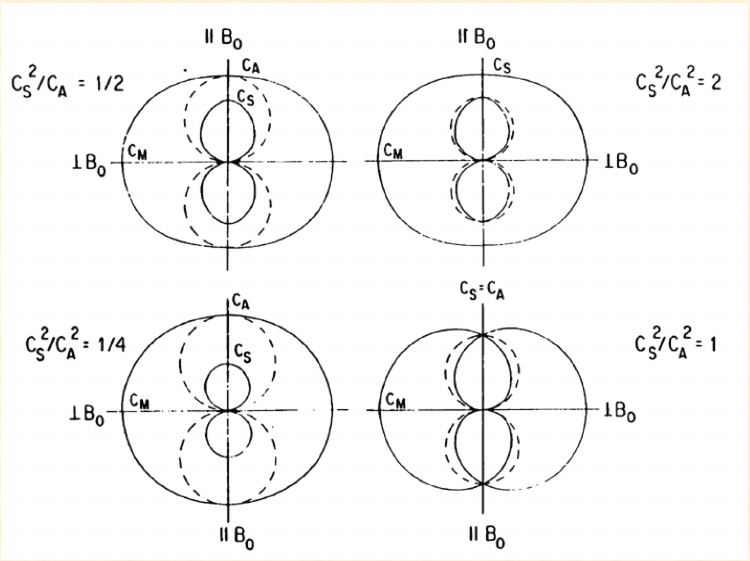
\includegraphics[width=0.8\textwidth]{Friedrichs.png}
  \caption{Friedrichs diagrams (from the slides)}
\end{figure}

However, the point of numerical simulations is to solve the full nonlinear
problem which can't be solved analytically. The simplest example is a contact
discontinuity: discontinuous change in density which constant $P$ advected at
constant $\mathbf{v}$. We can also have shocks where all variables can be
changed. In real life for example, when a plane flies across air at speed $v >
C$ it creates a shockwave. 

These kind of shocks are described by jump conditions, which are changes in
conserved variables across the discontinuity. To describe the hydrodynamic
shock, in the frame of the shock, there is a steady fluid flow toward the shock
from the upstream, and away from the show in the downstream direction. Mass,
energy and momentum are conserved in this frame. We can solve the equations for
the Rankine-Hugoniot jup conditions
\begin{equation}
  \label{eq:5}
  \frac{\rho_d}{\rho_u} = \frac{(\gamma + 1)\mathcal{M}^2}{(\gamma - 1)\mathcal{M}^2 + 2}
\end{equation}
where $M = v_u/C_u$ is the shock Mach number.

In MHD the shocks are more complicated since there are more kinds of shocks.
There can be Alfven ``shocks'' where only the transverse components of $v$ and
$B$ change discontinuously. There can be slow or fast shock, switch-on/off
shocks. These are shocks with small parameter space but very useful to test
codes to see if these can be captured.

Going beyond shocks is a zoo of linear instabilities of MHD fluids. Some of the
most important instabilities are gravitational instability, thermal instability,
Rayleigh-Taylor instability (light fluid supporting a heavy fluid under
acceleration), Richtmyer-Meshkov instability, Kelvin-Helmholtz instability (two
fluids flowing shearing across each other), and magneto-rotational instability
(in accretion disks for example). All these instabilities are important in
astrophysical conditions so we need to capture these correctly. Instabilities
often lead to turbulence, and the study of nonlinear turbulence is an important
application of the codes.

What do we mean by correctly? We need to understand what is feasible and what is
not. The dispersion relation for most MHD instabilities are unstable for a broad
range of wave numbers. However on a grid we can only have a finite resolution
depending on the grid size. Correctly means the linear growth rate of all modes
between $N\Delta x$ and $L$ are represented accurately. If we are studying
unresolved flows that is dominated by truncation error then we will get
different answer with different resolutions.

\subsection{Numerical Methods}

Lets start off by round-off error. Not all floating numbers can be represented
due to finite bit length. Rounding is correct if no machine number lies between
$x$ and its rounded value $x'$, and the difference between them is the round-off
error.

We can prove that the relative error of a rounded value is always bounded by a
small, machine dependent number
\begin{equation}
  \label{eq:6}
  \frac{|x - x'|}{|x|} < \epsilon
\end{equation}
which is the basis of all rigorous error analysis of numerical methods.

Another error is the truncation error. Numerical algorithms approximate analytic
solutions with algebraic operations. The difference between true and approximate
(numerical) solutions is the truncation error. This is under programmer control,
as oppose to the round-off error.

There are three concepts in numerical analysis that are very important:
Convergence, Consistency, and Stability. Convergence means when $\Delta x$ and
$\Delta t$ decreases, the truncation error should also decrease. Higher order
schemes often converge faster, but they cost more which puts a practical limit
on the usefulness of high order schemes. All methods are first-order for
discontinuities, so high order schemes are not very useful for shock capturing.

Consistency is another important concept which is often forgotten. It means that
the solutions of the underlying PDEs should not only converge but also converge
to the correct analytic solution. Finally stability is also important and it
means that round-off error must remain small and bounded. A solution can be
numerically unstable seeded by uncontrolled round-off error and it can grow
exponentially, which is undesirable.

The simplest discretization of a simple hyperbolic PDE is the forward-time
centered-space (FTCS) finite differencing method.
\begin{equation}
  \label{eq:7}
  \frac{\partial u}{\partial t} + a\frac{\partial u}{\partial x} = 0,\Longrightarrow \frac{u_j^{n+1} - u_j^n}{\Delta t} + a \left( \frac{u_{j+1}^n - u_{j-1}^n}{2\Delta x} \right) = 0
\end{equation}
We can perform a von Neumann stability analysis to show that this method is
unconditionally unstable. To show this we can insert
\begin{equation}
  \label{eq:8}
  u_j^n = \xi^n\exp(ikj\Delta x)
\end{equation}
When we substitute this into the finite difference equation we get $\xi(k) = 1 -
i(a\Delta t/\Delta x)\sin k\Delta x$. The amplitude of $\xi(k) > 0$ for all
$\Delta t > 0$. Therefore the method will blow up for any evolution in time.

However this is easy to fix by changing the time derivative to use an average of
$u$ at $t^n$ (Lax-Friedrichs):
\begin{equation}
  \label{eq:9}
  \frac{u_j^{n+1} + (u_{j+1}^n + u_{j-1}^n)/2}{\Delta t} + a \left( \frac{u_{j+1}^n - u_{j-1}^n}{2\Delta x} \right) = 0
\end{equation}
Now if we do the same analysis then we see $\xi(k) < 1$ iff
\begin{equation}
  \label{eq:10}
  \frac{a \Delta t}{\Delta x} \leq 1
\end{equation}
which is known as the Courant-Levy-Friedrichs (CFL) stability criterion.

Why does this work? In fact this LF equation introduces explicit numerical
viscosity which makes the algorithm stable, since we can rewrite the finite
difference equation to be %TODO

However the LF method has huge diffusion, so not recommended for practical use
nowadays. Another way is to use the Upwind methods
\begin{equation}
  \label{eq:11}
  \begin{split}
  \frac{u_j^{n+1} - u_j^n}{\Delta t} =&
    -a \left( \frac{u_j^n - u_{j-1}^n}{\Delta x} \right), \quad \text{if }a > 0 \\
    &-a \left( \frac{u_{j+1}^n - u_j^n}{\Delta x} \right), \quad \text{if }a < 0
  \end{split}
\end{equation}
This method has less diffusion than LF.

Both the above methods are diffusion methods. They add diffusion error to the
result, such that a localized perturbation will tend to diffuse away. Some other
methods (e.g. LW) will add dispersion error (with different dispersion
relation). Diffusion errors are acceptable, but dispersion errors will be
disastrous in some situations and should be avoided at all cost.

\subsection{Finite Volume Methods}

There is a zoo of algorithms for MHD. To list some of them: Finite-differencing
with hyper-viscosity, operator split methods, finite-volume methods, spectral
methods, discontinuous Galerkin methods, MHD SPH methods.

Finite volume MHD codes are popular and there are a variety of them: Athena,
VAC, AstroBEAR, PLUTO, FLASH, HARM, Enzo, Cosmo++, etc. This lecture will focus
on the methods in Athena.

\subsubsection{Discretization}

How does finite volume discretization work? We first discretize the space
$\mathbf{x} \rightarrow (x_i, y_i, z_i)$. We discretize time into $t \rightarrow
t^n$. We discretize continuous variables to be volume average values for each
cell. This is an important facet of the scheme, since it is not a sampling, but
an averaging.

We use a staggered mesh where scalars are cell-centered and magnetic fields are
defined at cell faces. Cell-centered quantities are volume-averaged and face
centered quantities are area-averaged. Since we mostly compute the curl of $B$,
area averaging is the natural discretization of the magnetic field.

We write the conservation laws in the form of hyperbolic equations
\begin{equation}
  \label{eq:12}
  \frac{\partial \mathbf{U}}{\partial t} + \frac{\partial \mathbf{F}}{\partial x} + \frac{\partial \mathbf{G}}{\partial y} + \frac{\partial \mathbf{H}}{\partial z} = 0
\end{equation}
We can integrate the equation over the volume of a grid cell, and over a
timestep $dt$, we can get an exact finite difference equation, where the
differences are differences over average values.

For the induction equation we use the finite area discretization, which is a
similar concept, but averaging over an area instead of a volume, which is
natural for the equation. Again we obtain an exact equation.

To summarize, mass, momentum, and energy fields are cell-centered. Fluxes are
face centered, and EMFs are edge-centered. The key is now to compute these
fluxes and EMFs all at once!

\subsubsection{Godunov Method}

The answer is to use Godunov's method. Difference in cell-averaged values at
each grid interface define a set of Riemann problems (evolution of initially
discontinuous states). The solution of Riemann problems averaged over cell gives
time evolution of cell-averaged values, until the wave hits the grid interfaces.
Due to conservation we don't even need to solve the Riemann problem exactly. We
only need to compute the flux through the interfaces between the cells, so we
only need to solve the Riemann problem at every cell interface.

So we introduce a Riemann solver. There are many possible solvers. In MHD
nonlinear Riemann solvers are complex because of the many families of waves and
many characteristics. In addition, the equations of MHD are not strictly
hyperbolic. Therefore MHD Gudonov schemes use approximate or linear Riemann
solvers.

There is Roe's method which keeps all 7 characteristics but treat each as a
simple wave. There is HLLE method which keeps only the largest and smallest
characteristics, but averages intermediate states in-between. There is also the
HLLC method which adds entropy and Alfven waves back into the HLLE method giving
2(4) intermediate states.

To determine which Riemann solver is the best, one needs to explore the use of
each. However the use of a Riemann solver is a benefit, not a weakness, since it
makes shock capturing more accurate: we encode in the numerical scheme a inherit
way of dealing with discontinuities.

We can use higher order methods to define Riemann problems to reconstruct
left-right states within cells using piecewise linear/parabolic methods. If we
need to do multidimensions, typically one split the equations directionally. One
solve the equations in $x$ directions first, then do it for $y$ with results
from the $x$ update, and so on. However in MHD this kind of splitting will not
preserve $\nabla\cdot \mathbf{B} = 0$. One needs to use directionally unsplit
methods. One first computes first order fluxes at every interface, use these
fluxes to advance solution for $\Delta t/2$, compute L/R states using this
time-advanced state, and fluxes, and then finally advance solutions over a full
timestep using the new fluxes.

\subsubsection{Constraints and Tests}

We also need to specify boundary conditions. Most codes apply boundary
conditions using ghost/guard cells.

How do we keep $\nabla\cdot \mathbf{B} = 0$? There are many ways. One way is to
do nothing and assume everything is okay. One way is to evolve $B$ using vector
potential $\mathbf{A}$, but this requires second derivatives which can be
numerically dangerous. One way is to remove solenoidal part of $\mathbf{B}$
using flux-cleaning, by setting $\mathbf{B} \to \mathbf{B} - \nabla\phi$ and
solving an elliptic PDE at every time step. Finally the way used in Athena is to
evolve the integral form of induction equation with Constrained Transport so
that $\nabla\cdot \mathbf{B} = 0$ is automatically conserved.

However the last CT method requires $E$ field at grid cell centers while they
are defined on edges. Arithmetic averaging destroys the scheme so we need an
algorithm to reconstruct $E$ field at the corner.

For stability we have to observe the CFL condition
\begin{equation}
  \label{eq:13}
  \Delta t \leq \frac{\Delta t}{v + C}
\end{equation}
We define the Courant number $C$ to be the ratio between lhs and rhs. For
stability we need $C<1$, and for multidimensions we usually need $C <
1/N_\text{dim}$.

There are many ways to test correctness. One simple way is to test linear wave
convergence in 3D. We measure the RMS error in $\mathbf{u}$ after propagating
a pure eigenmode for one wavelength. The error better decrease linearly with
increasing resolution. Some other tests include nonlinear circularly polarized
Alfven waves, shocktubes, MHD instabilities, etc.

\section{Lecture 2 --- Numerical Radiation MHD}

Numerical MHD is a relatively mature field, and there are quite a few public
codes that run well. However radiation MHD is still a very active field with
almost no consensus method at all. We will talk about what is Radiation MHD, and
numerical methods that we use.

\subsection{Radiation Hydrodynamics}

MHD is essential in black hole accretion disks, because angular momentum
transport is driven by MHD turbulence! However if we are talking about accretion
onto luminous sources, we need to consider radiation as well inside radius
(Shakura \& Sunyaev 1973)
\begin{equation}
  \label{eq:4}
  r/r_{g} < 170(L/L_\mathrm{Edd})^{16/21}(M/M_{\odot})^{2/21}
\end{equation}
Radiation pressure needs to be included in dynamic models. Radiation dominated
disks are subject to various instabilities, e.g.\ viscous instability and
thermal instability.

Foundations of Radiation Hydrodynamics is a good book. The challenges in this
field include:
\begin{itemize}
\item Which equations do we solve? Transfer equation vs. its moments.
    \item Which frame do we solve the equations in? Co-moving frame vs. Eulerian
      frame vs. mixed
    \item We need a proper closure of moment equations
    \item In diffusion limit the equations are hyperbolic-parabolic,
      mathematically challenging
    \item Wide range of timescales
    \item Frequency dependence adds another dimension
    \item Non-LTE effects requires modeling level populations
\end{itemize}

Radiation hydro means different things to different people. In some case it just
means a source term in the energy equation which is an integral over all
frequencies and scattering angles, which is a heating/cooling term by radiation.
This could be done in Godunov scheme via operator splitting:
\begin{itemize}
\item Update flux divergence terms ignoring source terms
    \item Update source terms
\end{itemize}
It is relatively easy to add a cooling term like $\rho^2\Lambda(T)$. However if
we just add this term, then the code is subject to thermal instability. The
growth rate is largest at small scales therefore grid scale truncation errors
can quickly grow to make too much small scale structure. If one adds heat
conduction this can be suppressed. It is crucial that one adds heat conduction
to get an accurate solution.

Another application domain is ionizing radiation transport, e.g.\ studying the
growth of HII regions in ISM. Now in the energy equation we have the heating and
cooling terms, and in the mass conservation equation we have ionization and
recombination terms. To add these ionization terms we need to compute radiative
transfer from every grid cell, which is a big challenge.

One way is to use the adaptive ray-tracing method of Abel \& Wandelt (2002) and
Whalen \& Norman (2006). The challenge is parallelization.

Another class of problems in this domain is to consider momentum transfer
instead of energy transfer. One now needs to include momentum exchange in the
force equation. One application is line-driven winds (assuming gas is
isothermal). However, the challenge is that computing this exchange term can be
extremely difficult!

Finally one might need to do the most general problem with both energy and
momentum transfer. One need to close the equations with radiation field energy
and momentum equation. One could even replace photons with neutrinos and do
neutrino transport instead of photon transport, like in the core-collapse SNe
community. All of the above problems can be called ``radiation hydrodynamics'',
but the numerical methods required in each regime are very different. In the
following part of the lecture we will focus on the problem with both energy and
momentum transfer.

Fundamental description of the radiation field is the frequency dependent
transfer equation
\begin{equation}
  \label{eq:14}
  \frac{1}{c}\frac{\partial I_{\nu}}{\partial t} + \nabla\cdot(\mathbf{n} I_{\nu}) = j_{\nu} - \kappa_{\nu}I_{\nu}
\end{equation}
One needs to decide to solve this equation or solving the moment of the
equation. Even after choosing the equation we can choose our method to be either
grid method or particle method. Grid methods are usually more accurate and less
noisy, and particle methods (usually Monte Carlo) are usually very flexible and
embarassingly parallelizable.

The noise in Monte Carlo methods is a real problem. It gives about $1\%$ noise
which could excite sound waves and other instabilities in the fluid. The Monte
Carlo is also very expensive compared to grid-based methods. However MC is great
for GR-RT which is used in EHT imaging of black holes, because it is not a
radiation pressure dominated problem.

\subsection{Numerical methods for radiation hydro}

Lets look at the radiation moment equations
\begin{align}
  \frac{\partial\rho}{\partial t} + \nabla\cdot(\rho \mathbf{v}) &= 0 \\
  \frac{\partial (\rho \mathbf{v})}{\partial t} + \nabla\cdot(\rho \mathbf{v}\mathbf{c} + P + B^2/2 - \mathbf{B}\mathbf{B}) &= -PS_M \\
  \frac{\partial E}{\partial t} + \nabla\cdot \left[ (E + P)\mathbf{v} + (B^2/2)\mathbf{v} - \mathbf{B}(\mathbf{B}\cdot \mathbf{v}) \right]  &= -PC S_E \\
  \frac{\partial \mathbf{B}}{\partial t} - \nabla\times(\mathbf{v}\times \mathbf{B}) &= 0 \\
  \frac{\partial E_r}{\partial t} + C\nabla\cdot \mathbf{F}_r &= C S_{E} \\
  \frac{\partial \mathbf{F}_r}{\partial t} + C \nabla\cdot P_r &= C S_{M}
\end{align}

One problem we have is the closure of these equations, since in general we can't
assume the distribution function of photons is Maxwellian. One thing we can do
is to assume $\mathbf{P} = \mathbf{f}E$, where $\mathbf{f}$ is called the
Eddington tensor. The flux-limited diffusion method assumes that radiation flux
is given by Ficks's Law
\begin{equation}
  \label{eq:15}
  \mathbf{F} = \frac{c\lambda}{\chi}\nabla E
\end{equation}
where $\lambda(E)$ is limited to prevent super-luminal transport in optically
thin regions. The other choice is the so-called M1 closure which assume a
specific tensor from first principles by going into a frame of the fluid where
the flow is isotropic. The third choice is to compute the Eddington tensor
numerically which is called the variable Eddington tensor (VET) approach. One
solves the time-independent transfer equations using method of short
characteristics along $N_r$ rays per cell, and take quadrature to get the
tensor.

The flux-limited diffusion method reduces our problem to two-temperature
diffusion problem (Turner \& Stone 2001). The main pro is that it is easy to
solve, but it lost information about the direction of flux. It also does not
have radiation inertia, therefore allowing superluminal wave speeds, and it has
no radiation shear viscosity.

We need a flux limiter $\lambda(E)$ and the most popular one is
\begin{equation}
  \label{eq:16}
  \lambda(R) = \frac{2 + R}{6 + 3R + R^2},\quad R = \left| \nabla E \right|/E
\end{equation}
which gives correct flux in both optically thin and optically thick limits.

Material radiation interaction and radiation transport terms have a very
restrictive time step limit, so we need to use implicit scheme for the
timestepping. The equations give sparse banded matrices which need to be solved
every NR iteration. There are iterative methods like GMRES or ICCG. This problem
is even worse in 3D. The challenge of doing flux-limited diffusion is solving
linear algebra problems.

There are approaches to get around this problem by reducing the speed of light
in the medium. Since the flow speed in the ISM is way smaller than $c$ we can
make the gap artificially smaller and solve the problem explicitly. However one
can derive constraints on slowest speed allowed to give correct dynamics
(Skinner \& Ostriker 2013).

Lets now consider M1 closure. It is a much improved method over FLD (Gonzalez
et.\ al.\ 2007). It keeps flux as a separate variable and uses local information
to construct direction of flux. This fixes the shadowing problem with FLD, but
replaces with photons colliding and merging problem. Photons behave like a
collective fluid rather than particles, because M1 assumes there is a frame
where the flow is isotropic while in reality there might not be. M1 is usually
more attractive when there is a small number of sources.

Finally there is the VET approach (Trujillo Bueno \& Fabiani Bendicho 1995). One
could use short characteristics method solving only along ray segments that
cross a single zone, or one could use long characteristics where we solve along
rays that cross entire grid for each cell. Long characteristics are usually not
feasible, but short characteristics can have problems in treating point sources,
e.g.\ having spikes away from point sources which breaks symmetry.

\subsection{Radiation in Godunov methods}

Lets now consider how to put this into Godunov method. Assuming we have picked a
scheme to solve the closure problem, we still face the problem of solving the
Godulov method with stiff source terms. One could use semi-implicit (Picard
iteration) schemes to ensure stability.

When one consider long evolutions we might want to use implicit methods anyway,
but it can be expensive and inaccurate. Instead we could split fully implicit
solution of the radiation moment equations from modified Godunov method for MHD
equation, and we write our own implicit solvers for the moment equations.

A test for the full code is the classic linear wave convergence test. One could
write down the linear waves of this system (quite nontrivial) and we can test
the convergence to analytic solution in 3D with respect to grid resolution.

One also need to do nonlinear tests since linear tests don't make use of all
terms. One nonlinear test would be radiation shock tests. In radiation hydro one
could have a precursor region which is heated up by the photons, and in the
post-shock gas might cool (relaxation region) due to photons leaving. This
structure depends on the Mach number. The particle mean free path and photon
mean free path are two scales which can be very very different. Getting the
shock structure is pretty difficult (semi)analytically.

The cost of 3D RMHD equations using explicit differencing scales as
$N_xN_yN_zN_mN_n$ where $N_m$ is number of angles, and $N_n$ is the number of
frequencies. However this admits very efficient parallelization. One could also
use adaptive angles and frequencies could be very powerful.




\end{document}
